% Exact LaTeX recreation of the supplied Phase-1.pdf
% Compile with pdfLaTeX. Place member pictures in the same folder if required.

\documentclass[11pt,a4paper]{article}

\usepackage[a4paper,left=2.0cm,right=2.0cm,top=1.55cm,bottom=1.55cm]{geometry}
\usepackage[T1]{fontenc}
\usepackage{lmodern}
\usepackage{graphicx}
\usepackage{xcolor}
\usepackage{array}
\usepackage{tabularx}
\usepackage{ragged2e}
\usepackage{enumitem}
\usepackage{fancyhdr}
\usepackage{tikz}
\usepackage{setspace}

% -------------------------------------------------
% COLOURS
% -------------------------------------------------
\definecolor{TitleBlue}{RGB}{61,103,154}

% -------------------------------------------------
% GENERAL SETTINGS
% -------------------------------------------------
\setlength{\parindent}{0pt}
\setlength{\parskip}{0pt}
\renewcommand{\arraystretch}{1.0}

% The supplied document uses a clean sans-serif heading style
% and italic serif-style explanatory text.
\newcommand{\blueheading}[1]{%
    {\sffamily\color{TitleBlue}\fontsize{15}{18}\selectfont #1}%
}

\newcommand{\bluebigheading}[1]{%
    {\sffamily\bfseries\color{TitleBlue}\fontsize{16}{19}\selectfont #1}%
}

\newcommand{\instruction}[1]{%
    {\itshape\fontsize{10.5}{12.5}\selectfont #1}%
}

\newcommand{\answerbox}[2][3.0cm]{%
    \vspace{2pt}
    \noindent
    \fbox{%
        \begin{minipage}[t][#1][t]{\dimexpr\textwidth-2\fboxsep-2\fboxrule\relax}
            \vspace{1mm}
            \itshape #2
        \end{minipage}
    }
}

% -------------------------------------------------
% HEADER / FOOTER
% -------------------------------------------------
\pagestyle{fancy}
\fancyhf{}
\renewcommand{\headrulewidth}{0pt}
\renewcommand{\footrulewidth}{0pt}

\fancyhead[L]{%
    \sffamily\bfseries\itshape\fontsize{10.5}{12}\selectfont
DSCPP-III-2026-T014
}
\fancyhead[R]{%
    \sffamily\bfseries\fontsize{10.5}{12}\selectfont
    PROJECT PROPOSAL
}
\fancyfoot[R]{%
    \itshape\fontsize{10}{12}\selectfont
    Page \thepage
}
\setlength{\headheight}{14pt}
\setlength{\headsep}{23pt}
\setlength{\footskip}{24pt}

% -------------------------------------------------
% PAGE 1
% -------------------------------------------------
\begin{document}

\vspace*{4mm}

\bluebigheading{PROJECT AND TEAM INFORMATION}

\vspace{13mm}

\blueheading{Project Title}

\vspace{1mm}

\instruction{}

\answerbox[1.0cm]{SheShield: A Safety Navigation System}

\vspace{13mm}

\blueheading{Student / Team Information}

\vspace{2mm}

% Team information table
% Compact 4-member layout so all members remain on Page 1.
\noindent
\begin{tabularx}{\textwidth}{|>{\RaggedRight\arraybackslash}p{0.69\textwidth}|>{\RaggedRight\arraybackslash}X|}
\hline
\begin{minipage}[t]{\linewidth}
\vspace{1.5mm}
\textit{Team Name:}\\[-1mm]
\textit{Team \#}
\vspace{1.5mm}
\end{minipage}
&
\begin{minipage}[t]{\linewidth}
\vspace{1.5mm}
\textit{NextGen}
\vspace{1.5mm}
\end{minipage}
\\
\hline
\begin{minipage}[t][3.25cm][t]{\linewidth}
\vspace{1.5mm}
\textbf{Team member 1 (Team Lead)}\\[-1mm]
\textit{(Last Name, name: student ID: email, picture):}
\vspace{2.0cm}
\end{minipage}
&
\begin{minipage}[t][3.25cm][t]{\linewidth}
\vspace{1.5mm}
\textit{Aditi -- 2510019093}\\
\textit{@adititomarrr18@gmail.com}

\vspace{2mm}
\includegraphics[width=3.0cm,height=1.5cm,keepaspectratio]{ad.png}
\end{minipage}
\\
\hline
\begin{minipage}[t][3.25cm][t]{\linewidth}
\vspace{1.5mm}
\textbf{Team member 2}\\[-1mm]
\textit{(Last Name, name: student ID: email, picture):}
\vspace{2.0cm}
\end{minipage}
&
\begin{minipage}[t][3.25cm][t]{\linewidth}
\vspace{1.5mm}
\textit{Kohli, Dakshi -- 2510010454}\\
\textit{kohlidakshi90@gmail.com}

\vspace{2mm}
\includegraphics[width=3.0cm,height=1.5cm,keepaspectratio]{dakshi.png}
\end{minipage}
\\
\hline
\begin{minipage}[t][3.25cm][t]{\linewidth}
\vspace{1.5mm}
\textbf{Team member 3}\\[-1mm]
\textit{(Last Name, name: student ID: email, picture):}
\vspace{2.0cm}
\end{minipage}
&
\begin{minipage}[t][3.25cm][t]{\linewidth}
\vspace{1.5mm}
\textit{Nehra, Vidit -- 251001187}\\
\textit{nehravidit07@gmail.com}

\vspace{2mm}
\includegraphics[width=3.0cm,height=1.5cm,keepaspectratio]{v.png}
\end{minipage}
\\
\hline
\begin{minipage}[t][3.25cm][t]{\linewidth}
\vspace{1.5mm}
\textbf{Team member 4}\\[-1mm]
\textit{(Last Name, name: student ID: email, picture):}
\vspace{2.0cm}
\end{minipage}
&
\begin{minipage}[t][3.25cm][t]{\linewidth}
\vspace{1.5mm}
\textit{Pundir, Avni -- 2510011647}\\
\textit{avnipundir2007@gmail.com}

\vspace{2mm}
 \includegraphics[width=3.0cm,height=1.5cm,keepaspectratio]{av.png}
\end{minipage}
\\
\hline
\end{tabularx}

\newpage

% -------------------------------------------------
% PAGE 2
% -------------------------------------------------

\bluebigheading{PROPOSAL DESCRIPTION (10 pts)}

\vspace{12mm}

\blueheading{Motivation (1 pt)}

\vspace{1mm}

\instruction{(Describe the problem you want to solve and why it is important. Max 300 words).}

\answerbox[3.0cm]{
The major issue with current navigation applications is that they prioritize the shortest or fastest route instead of focusing on the safety of female travelers. Additionally, during emergency situations, these applications require the user to have multiple applications for SOS alerts, live tracking, and trusted contacts that can be contacted for help
Hence, the motivation behind our project is to propose a women-focused system that offers a safe route, SOS, live tracking, and trusted contacts in one application.

}

\vspace{12mm}

\blueheading{State of the Art / Current solution (1 pt)}

\vspace{1mm}

\instruction{(Describe how the problem is solved today (if it is). Max 200 words).}

\answerbox[2.75cm]{
As mentioned above, women have to rely on standard navigation applications where the routes are prioritized on the basis of the distance or time instead of focusing on the safety of the traveler. Additionally, SOS, live tracking, and trusted contacts are available through separate applications.
Although some applications offer safety features, they do not integrate them with the core navigation system, which should be the primary focus of any woman-focused application. Hence, our project focuses on integrating Safe Route, SOS, Live Location Sharing, and Trusted Contacts into one application.

}

\vspace{12mm}

\blueheading{Project Goals and Milestones (2 pts)}

\vspace{1mm}

\instruction{(Describe the project general goals. Include initial milestones as well any other milestones. Max 300 words).}

\answerbox[3.15cm]{
Our project’s primary objective is to propose a woman-focused safety navigation system that utilizes graph algorithms in order to prioritize the safe route while also offering SOS, live location sharing, and trusted contacts.
The following are the major goals of our project:
1. Develop a women-focused safety navigation system that utilizes graph-based algorithms to determine the safe route while also prioritizing emergency SOS, live tracking, and trusted contacts.
2. Implement the Safe Route, SOS, Live Location Sharing, and Trusted Contacts features and test/debug before finalizing the documentation.
}

\vspace{12mm}

\blueheading{Project Approach (3 pts)}

\vspace{1mm}

\instruction{(Describe how you plan to articulate and design a solution. Including platforms and technologies that you will use. Max}

\instruction{300 words).}

\answerbox[3.05cm]{
1. Safe Route will utilize graphs and Dijkstra’s Algorithm in order to determine the safe route.
2. SOS, Live Location Sharing, and Trusted Contacts will offer an easy way to contact emergency contacts while also live tracking the user’s location.
3. C++ will be used to implement the core logic of the application which revolves around graphs, arrays, vectors, queues, and searching algorithms. The console application will be a prototype of the actual application with basic features.
4. Graphs will be used to implement the Safe Route feature using Dijkstra’s Algorithm.
}

\newpage

% -------------------------------------------------
% PAGE 3
% -------------------------------------------------

\blueheading{System Architecture (High Level Diagram)(2 pts)}

\vspace{1mm}

\instruction{(Provide an overview of the system, identifying its main components and interfaces in the form of a diagram using a tool}

\instruction{of your choice).}

\answerbox[4.0cm]{
    \centering
    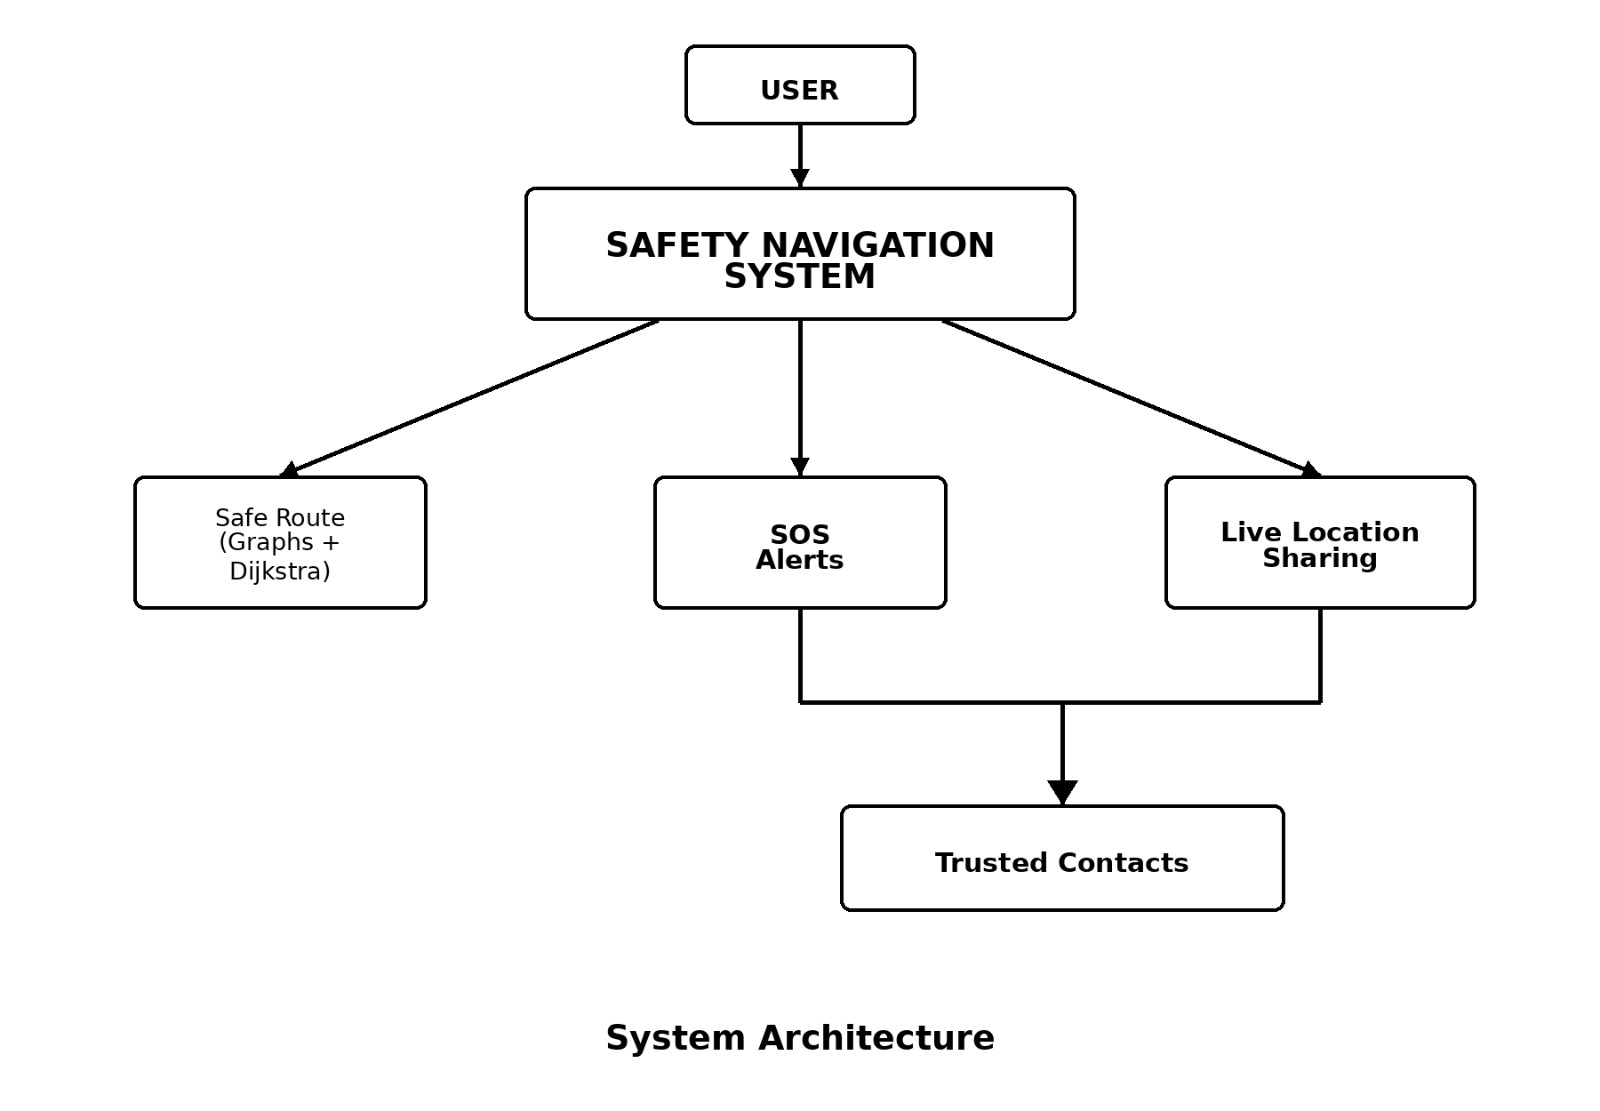
\includegraphics[
        width=0.95\textwidth,
        height=3.5cm,
        keepaspectratio
    ]{use.png}
}


\vspace{12mm}

\blueheading{Project Outcome / Deliverables (1 pts)}

\vspace{1mm}

\instruction{(Describe what are the outcomes / deliverables of the project. Max 200 words).}

\answerbox[2.7cm]{
The outcome of our project will be a prototype of the women-focused safety navigation system that will offer Safe Route, SOS, Live Location Sharing, and Trusted Contacts. In addition, this project will highlight the importance of utilizing C++ and Data Structures & Algorithms to address real-time problems.

The final deliverables of our project will include the prototype application, source code, system documentation, and test results.

}

\vspace{12mm}

\blueheading{Assumptions}

\vspace{6mm}

\instruction{( Describe the assumptions ( if any ) you are making to solve the problem. Max 100 words )}

\answerbox[2.65cm]{The project will assume that the user has a device with location services enabled and has added emergency contacts to the application. For the prototype, it can be assumed that the route information will be static instead of using actual maps and location services to determine the route. It also assumes that the user has an active internet connection in order to use the live tracking and emergency contact features. The safe route feature will be determined using the given information and should not be used as a reliable indicator of the actual safe route.}

\vspace{12mm}

\blueheading{References}

\vspace{1mm}

\instruction{(Provide a list of resources or references you utilised for the completion of this deliverable. You may provide links).}

\answerbox[2.65cm]{C++ Documentation - For reference to C++ concepts, functions, and implementation.

GeeksforGeeks - For reference to Graphs, Dijkstra’s Algorithm, and Data Structures.

Programiz - For reference to C++ and Data Structures.

Google Maps - For reference to current route navigation and location services.

Research articles and online resources on women’s safety and emergency applications - For reference to current applications and potential features that can be integrated.}

\end{document}
